\section{Create 3D Mask protocol}
\label{app:create3DMask}%a061

Protocol designed to create a mask, $i.e.$, a wrapping surface able to delimit a volume or subunit of interest, in order to modify the density values within or outside it. This mask can be created with a given geometrical shape (sphere, cube, cylinder...) or obtained from operating on a 3d volume or a previous mask.

\begin{itemize}
 \item Requirements to run this protocol and visualize results:
    \begin{itemize}
        \item \scipion plugin: \ttt{scipion-em-xmipp}
    \end{itemize}
 \item \scipion menu:\\
  \ttt{Model building -> Preprocess map} (\ffigure{fig:create3DMask_1} (A))
  
 \item Protocol form parameters (\ffigure{fig:create3DMask_1} (B: Mask generation; C: Postprocessing)):
  
    \begin{figure}[H]
     \centering 
     \captionsetup{width=.7\linewidth} 
     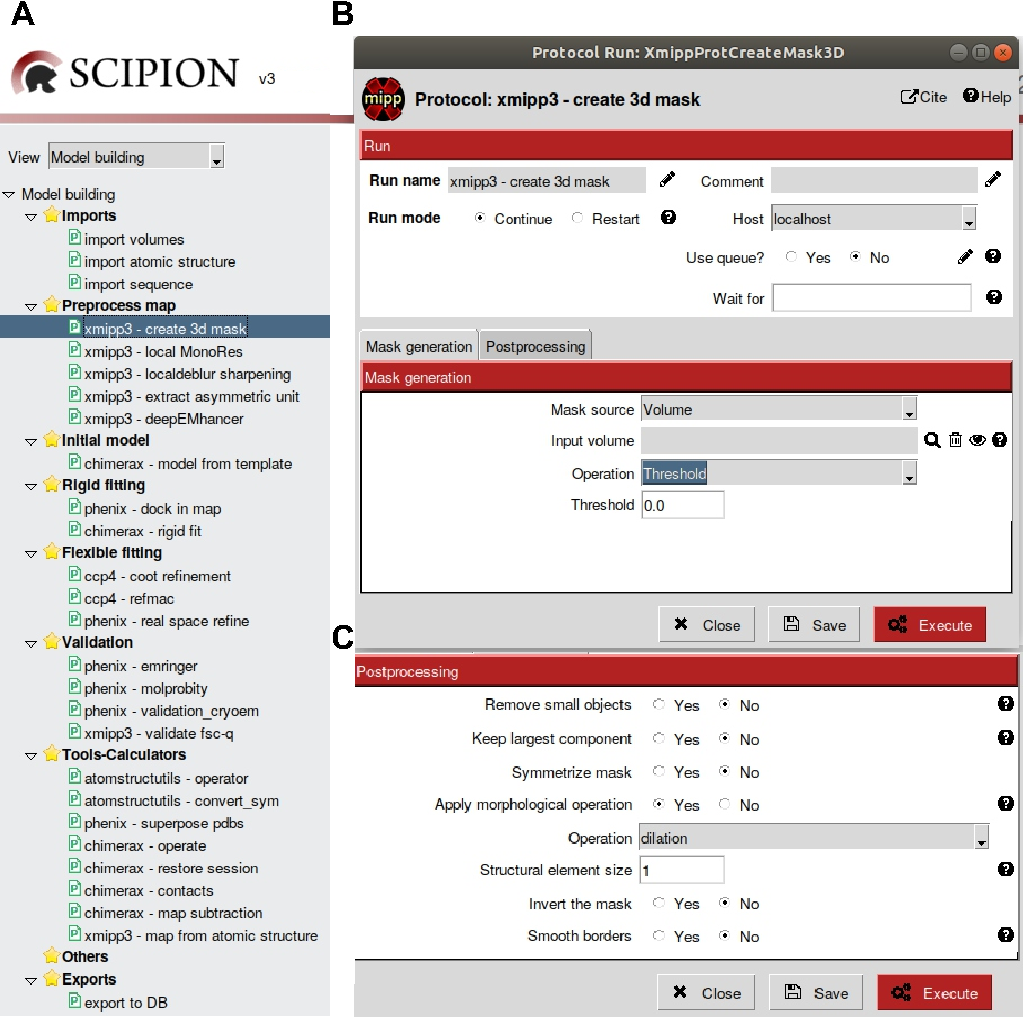
\includegraphics[width=0.90\textwidth]{Images_appendix/Fig206}
     \caption{Protocol \scommand{xmipp3 - create 3d mask}. A: Protocol location in \scipion menu. B, C: Protocol form.}
     \label{fig:create3DMask_1}
    \end{figure}
    
    \begin{itemize}
     \item \ttt{Mask generation}
     \begin{itemize}
      \item \ttt{Mask source}: Selection of one of the two possible types of sources for the mask, the map volume provided by the user or a specific geometrical design.\\If a volume is selected:
        \begin{itemize}
        \item \ttt{Input volume}: Electron density map previously downloaded or generated in \scipion.
        \item \ttt{Operation}: Approach applied to generate the mask, besides methods that can be selected in Postprocessing, such as establishing a particular density \ttt{threshold}, a segmentation process according to the number of voxels, number of aminoacids, atomic mass (Daltons) or automatic.
        \end{itemize}
      If a geometric shape is selected:
        \begin{itemize}
        \item \ttt{Sampling Rate (\AA\/px)}: Size of voxel dimensions in \AA.
        \item \ttt{Mask size (px)}: Mask dimensions in number of pixels.
        \item \ttt{Mask type}: Sphere, box, crown, cylinder, Gaussian, raised cosine and raised crown. Dimensions of each one of these geometric shapes have to be assigned in pixels: Radius of the sphere (half size of the mask by default); box size; inner and outer radius of the crown, raised cosine and raised crown (half size of the mask by default); height of cylinder (mask size by default); Gaussian sigma (mask size/6 by default); and border decay or fall-off of the two borders of the crown (0 by default).
        \end{itemize}  
      \item \ttt{Shift center of the mask?}: By selecting ``Yes'', the mask will be shifted to a new origin of coordinates \ttt{X, Y, Z}.
     \end{itemize} 
     \item \ttt{Postprocessing}
     \begin{itemize}
     \item \ttt{Remove small objects}: Selection of ``Yes'' allows to ignore ligands of the map volume below a certain size (in voxels).
     \item \ttt{Keep largest component}: By selecting ``Yes'' a mask will be generated considering only the largest element of the map volume, ignoring the rest.
     \item \ttt{Symmetrize mask}: By selecting ``Yes'' a symmetrized mask will be generated according to a specific symmetry group (look at http://xmipp.cnb.csic.es/twiki/bin/view/Xmipp/Symmetry). \ttt{c1} symmetry indicates no symmetry, by default.
     \item \ttt{Apply morphological operation}: Slight modifications of the mask can be applied by dilation or erosion of the density region (\ttt{Structural element size}: One voxel by default). Combinations of dilation and erosion allow closing or opening empty spaces of density in the map volume.
     \item \ttt{Invert the mask}: This option allows to invert the values of density regarding the wrapping surface of the mask, masking the outer part instead the inner part.
     \item \ttt{Smooth borders}: Mask borders can be smoothed by applying a convolution of the mask with a Gaussian. The Gaussian sigma (in pixels) has to be supplied.
     \end{itemize}

    \end{itemize}
 
 \item Protocol execution:\\
 Adding specific map/structure label is recommended in \ttt{Run name} section, at the form top. To add the label, open the protocol form, press the pencil symbol at the right side of \ttt{Run name} box, complete the label in the new opened window, press OK and, finally, close the protocol. This label will be shown in the output summary content (see below). If you want to run again this protocol, do not forget to set to \ttt{Restart} the \ttt{Run mode}.\\
  Press the \ttt{Execute} red button at the form bottom.
  
  \item Visualization of protocol results:
  
  After executing the protocol, press \ttt{Analyze Results} and $ShowJ$ (\url{https://github.com/I2PC/scipion/wiki/ShowJ}), the default \scipion viewer, will open the mask by slices. The $ShowJ$ window menu (\ttt{File -> Open with Chimera}) allows to open the mask volume in $Chimera$ graphics window.

 \item Summary content:
  \begin{itemize}
     \item Protocol output (below \scipion framework):\\ \ttt{xmipp3 - create 3d mask -> ouputMask}; VolumeMask (x, y, and z dimensions, sampling rate).
     \item \ttt{SUMMARY} box:\\ Details about \ttt{Mask creation} and \ttt{Mask processing}.
    \end{itemize}
    
 \end{itemize}
